\documentclass[xcolor=table,aspectratio=169]{beamer}
\usepackage{beamerthemesplit}
\usepackage{wrapfig}
\usetheme{SPbGU}
\usepackage{pdfpages}
\usepackage{amsmath}
\usepackage{cmap}
\usepackage[T2A]{fontenc}
\usepackage[utf8]{inputenc}
\usepackage[english]{babel}
\usepackage{indentfirst}
\usepackage{mathtools}
\usepackage{pgf}
\usepackage{soul}
\usepackage{tikz}
\usepackage{multirow}
\usepackage[noend]{algpseudocode}
\usepackage{algorithm}
\usepackage{algorithmicx}
\usepackage{fancyvrb}

\usepackage{minted}

\usetikzlibrary{shapes, arrows, automata, fit, calc, positioning}


\usepackage{fontawesome}

\usetikzlibrary{shapes.callouts}

\usepackage{xparse}

%for [[ ]]
\usepackage{stmaryrd}


\tikzset{
    invisible/.style={opacity=0,text opacity=0},
    visible on/.style={alt=#1{}{invisible}},
    alt/.code args={<#1>#2#3}{%
      \alt<#1>{\pgfkeysalso{#2}}{\pgfkeysalso{#3}} % \pgfkeysalso doesn't change the path
    },
}

\NewDocumentCommand{\mycallout}{r<> O{opacity=0.8,text opacity=1} m m m}{%
\tikz[remember picture, overlay]\node[align=center, fill=cyan!20, text width=#5cm,
#2,visible on=<#1>, rounded corners,
draw,rectangle callout,anchor=pointer,callout relative pointer={(230:1cm)}]
at (#3) {#4};
}

%\newcommand{\tikzmark}[1]{\tikz[overlay,remember picture,baseline=-0.5ex] \node (#1) {};}



\usepackage{tabularx}
\newcolumntype{Y}{>{\raggedleft\arraybackslash}X}

\renewcommand{\thealgorithm}{}

\newtheorem{mytheorem}{Theorem}
\renewcommand{\thealgorithm}{}

\newcommand{\tikzmark}[1]{\tikz[overlay,remember picture] \node (#1) {};}
\def\Put(#1,#2)#3{\leavevmode\makebox(0,0){\put(#1,#2){#3}}}

\newcommand{\ltz}{$< 1$}

\newcommand{\nodeDistanceRsm}{2.5cm}
\newcommand{\rsmInnerXSep}{0.1cm}
\newcommand{\rsmInnerYSep}{0.8cm}

\tikzset{
    state/.style={
           rectangle,
           rounded corners,
           draw=black, very thick,
           minimum height=2em,
           inner sep=2pt,
           text centered,
           },
}

\makeatletter
\AtBeginEnvironment{minted}{\dontdofcolorbox}
\def\dontdofcolorbox{\renewcommand\fcolorbox[4][]{##4}}
\makeatother

\beamertemplatenavigationsymbolsempty

\title[GLL-based CFPQ for Neo4j]{GLL-based Context-Free Path Querying for Neo4j}
%\subtitle[YaccConstructor]{Parsing techniques for graph analysis}
\institute[SPbSU]{
Saint Petersburg State University
}


\author[Semyon Grigorev]{Vadim Abzalov, Vlada Pogozhelskaya, Vladimir Kutuev, \\ Olga Bachishche, \textbf{Semyon Grigorev}}

\date{October 31, 2025}

\begin{document}
{
\begin{frame}[fragile]
  \begin{table}
  \centering
  \begin{tabularx}{\linewidth}{XcX}
    
\includegraphics[height=1.5cm]{pictures/damdid_logo.png} \hfill
    & \hfill %\begin{minipage}[t]{0.3\textwidth}\center \includegraphics[height=1.5cm]{pictures/EDBT.png} \hfill
      %\end{minipage}
    & \hfill 
\includegraphics[height=1.5cm]{pictures/SPbGU_Logo.png}
  \end{tabularx}
  \end{table}
  \titlepage
\end{frame}
}

\begin{frame}[fragile] \frametitle{Formal Language Constrained Path Querying}
      \begin{minipage}[m]{0.45\linewidth}
  \raisebox{-0.5\totalheight}{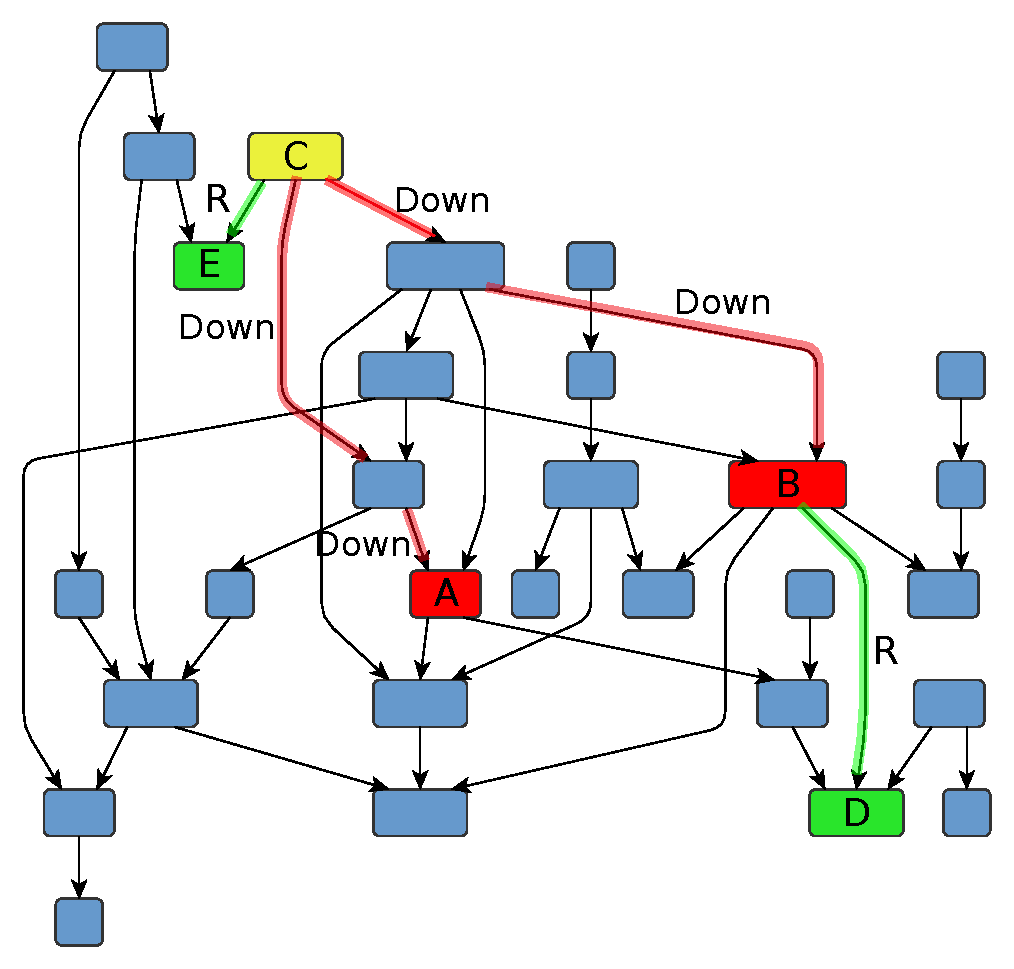
\includegraphics[width=\textwidth]{pictures/hierarchical_rpq.pdf}}
  \end{minipage}\hfill
  \begin{minipage}[m]{0.5\linewidth}
  Navigation through an edge-labeled graph

  \vfill

  \begin{itemize}
        \item \textbf{Path} specifies a \textbf{word} formed by the~labels of the edges
        \item \textbf{Paths constraint} is a \textbf{language}: the~word specified by the path should be in~the given language
        \item The expressiveness of constraints is related~to \textbf{formal languages classes}
  \end{itemize}
  \end{minipage}

\end{frame}


\begin{frame}[fragile] \frametitle{Regular Path Queries (RPQ)}
      \begin{minipage}[m]{0.45\linewidth}
  \raisebox{-0.5\totalheight}{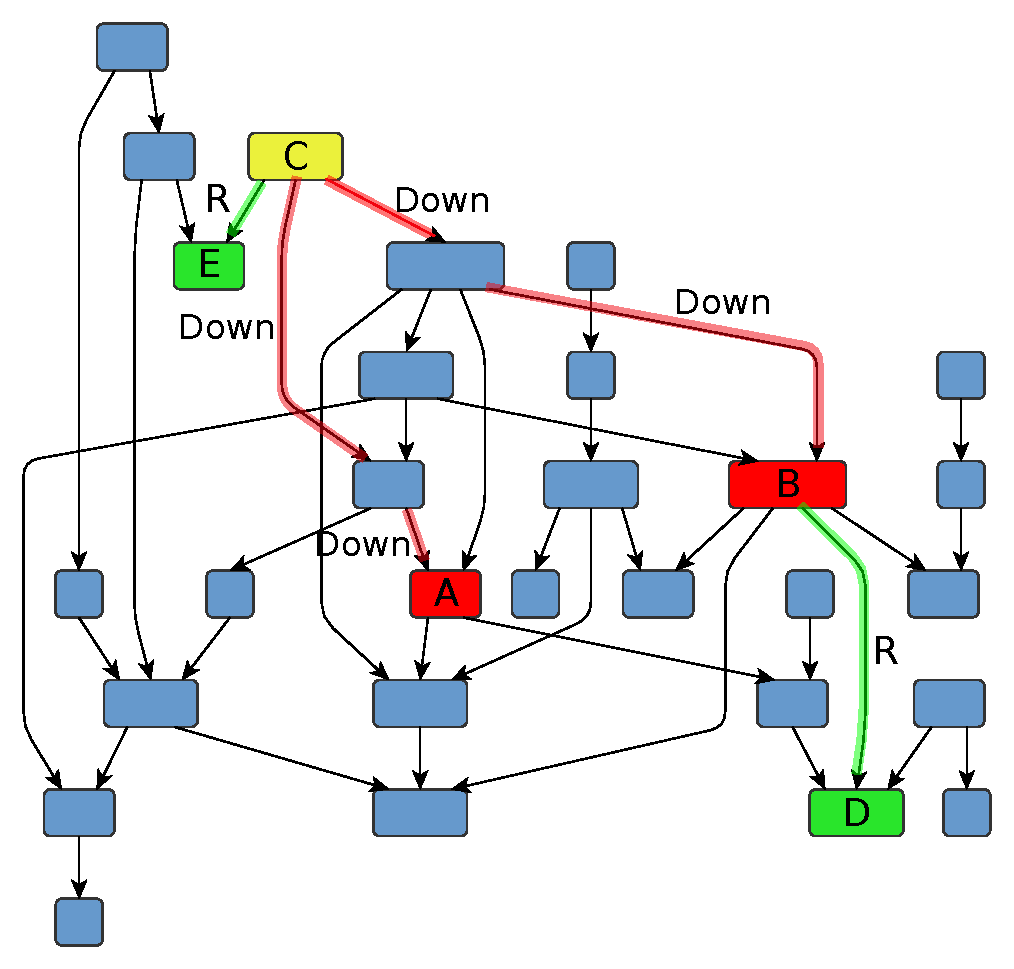
\includegraphics[width=\textwidth]{pictures/hierarchical_rpq.pdf}}
  \end{minipage}\hfill
  \begin{minipage}[m]{0.5\linewidth}
  \textbf{Regular} languages as constraints

  \vfill


  \begin{itemize}
        \item Which nodes are reachable from \textbf{C} by arbitrary number of $\textbf{R} \text{ and } \textbf{Down}$ edges?
        \item Regular language $\mathcal{L} = (\textit{R} \mid \textit{Down})^*$
  \end{itemize}
  \vspace{2cm}
  \begin{itemize}    
    \item Part of GQL and SQL/PGQ (ISO/IEC 9075-16:2023)
  \end{itemize}

  \end{minipage}

\end{frame}


\begin{frame}[fragile] \frametitle{Context-Free Path Queries (CFPQ)}
      \begin{minipage}[m]{0.45\linewidth}
  \raisebox{-0.5\totalheight}{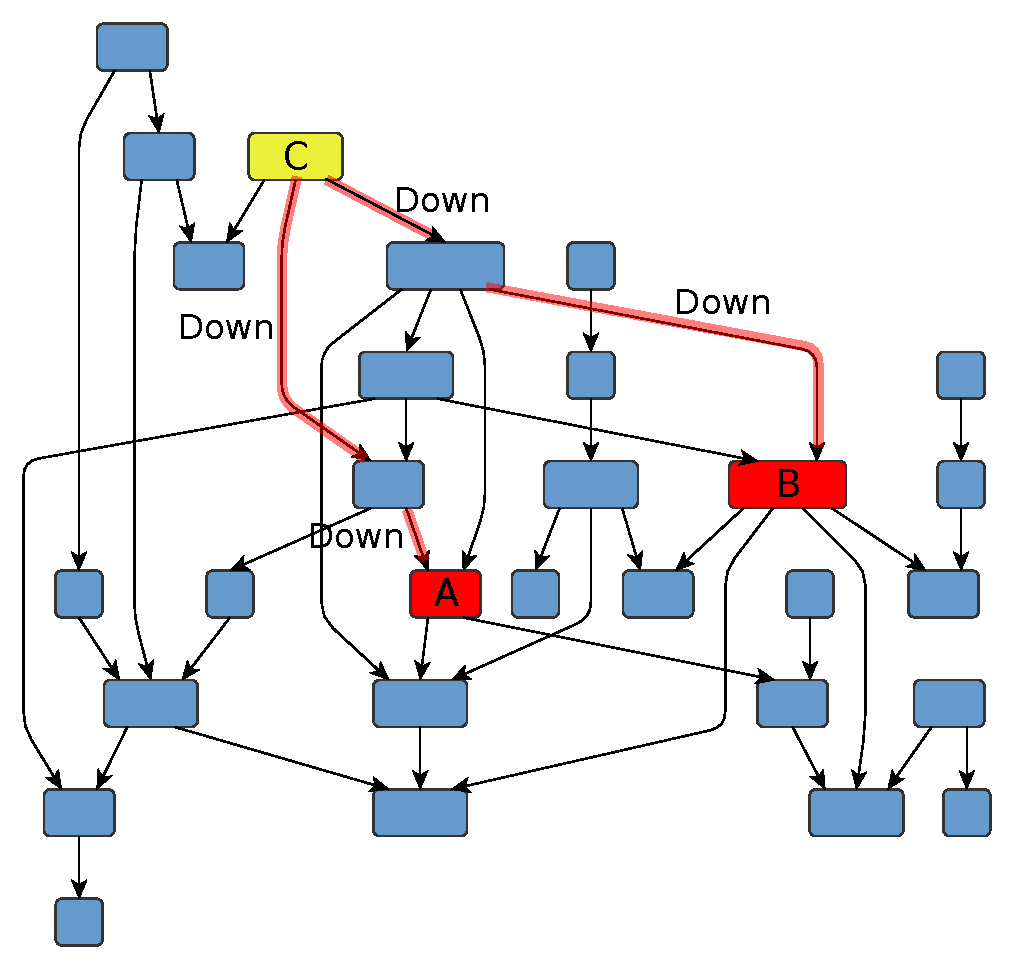
\includegraphics[width=\textwidth]{pictures/hierarchical.pdf}}
  \end{minipage}\hfill
  \begin{minipage}[m]{0.5\linewidth}
  \textbf{Context-free} languages as constraints
  \begin{itemize}
        \item Are nodes A and B on the same level of hierarchy?
        \item Is there a path of form $\overline{\textbf{Down}}^n \, \textbf{Down}^n$ between A and B?
        \item Context-free grammar: $\textit{SameLvl} \to \overline{\textit{Down}} \ \textit{SameLvl} \ \textit{Down} \mid \varepsilon$
  \end{itemize}
  \pause

  \vspace{0.3cm}


  Applications
    \begin{itemize}
      \item Static code analysis [\href{https://dl.acm.org/doi/10.1145/199448.199462}{T. Reps, et al, 1995}]
      \item Graph segmentation [\href{https://dblp.org/rec/conf/icde/0001D19.html}{H. Miao, et al, 2019}]
      \item Bio data analysis [\href{https://pubmed.ncbi.nlm.nih.gov/20134073/}{P. Sevon, et al, 2008}]
      \item \ldots
    \end{itemize}

  \end{minipage}

  \end{frame}

\begin{frame}[fragile] \frametitle{Problem Statement}
   \begin{itemize}
      \item J. Kuijpers, et al\footnote<.(1)->{Jochem Kuijpers, George Fletcher, Nikolay Yakovets, and Tobias Lindaaker. 2019. An Experimental Study of Context-Free Path Query Evaluation Methods.}: existing algorithms are too slow to be used in practical applications (in~the context of Neo4j)      
      \item Reachability in the focus
      \begin{itemize}
        \item Paths needed in some applications
        \item Not for all pairs, but for specified start vertices
      \end{itemize}
      \vfill
      \item[\faQuestion] How to create faster multiple source context-free all paths querying algorithm?
    \end{itemize}

\end{frame}


\begin{frame}[fragile] \frametitle{Proposed Solution}
  \begin{itemize}
      \item \textbf{Generalized LL (GLL)}\footnote{A. Afroozeh, Anastasia Izmaylova. Faster, Practical GLL Parsing. 2015} as a base
      \begin{itemize}
        \item Arbitrary grammars (including left-recursive and ambiguous) without transformations
        \item \textbf{Shared Packed Parse Forest (SPPF)} is a native representation of all paths
        \item Directed --- native support of source vertices
      \end{itemize}
      \item \textbf{Recursive State Machine (RSM)} to represent constraints
      \begin{itemize}
        \item Instead of grammar in (E)BNF\footnote{Right part of the rule is a regular expression over terminals and nonterminals}
      \end{itemize}
  \end{itemize}

\end{frame}


\begin{frame}[fragile] \frametitle{Definitions}
  \begin{itemize}
      \item \textbf{Descriptor} $d=(u,q,g)$ --- configuration of recognizer/parser
      \begin{itemize}
        \item $u$ --- vertex of the input graph
        \item $q$ --- state of the RSM (constraint)
        \item $g$ --- current top of the stack (vertex of GSS) 
      \end{itemize}
      \item \textbf{Graph Structured Stack (GSS)} --- compact\footnote{Cubic in worst case} representation of multiple stacks
      \begin{itemize}
        \item Vertex $(M,u)$ --- Handling of nonterminal $M$ is started from vertex $u$ of the input graph
        \item Each edge is labelled with $p$ --- state of the RSM to continue from after pop
      \end{itemize}
      \item \textbf{Shared Packed Parse Forest (SPPF)} --- compact\footnote{Cubic in worst case} representation of all possible derivation trees
      \begin{itemize}
        \item \textbf{Terminal} and \textbf{nonterminal} nodes
        \item \textbf{Packed, intermediate, etc} --- special nodes to reuse subtrees
      \end{itemize}
      \item \textbf{Recursive State Machine (RSM)} --- finite-automata-like representation of context-free language
      \begin{itemize}
        \item DFA representation of right part of rule for each nonterminal
      \end{itemize}
  \end{itemize}

\end{frame}

\begin{frame}[fragile] \frametitle{An Example}
  \begin{center}
      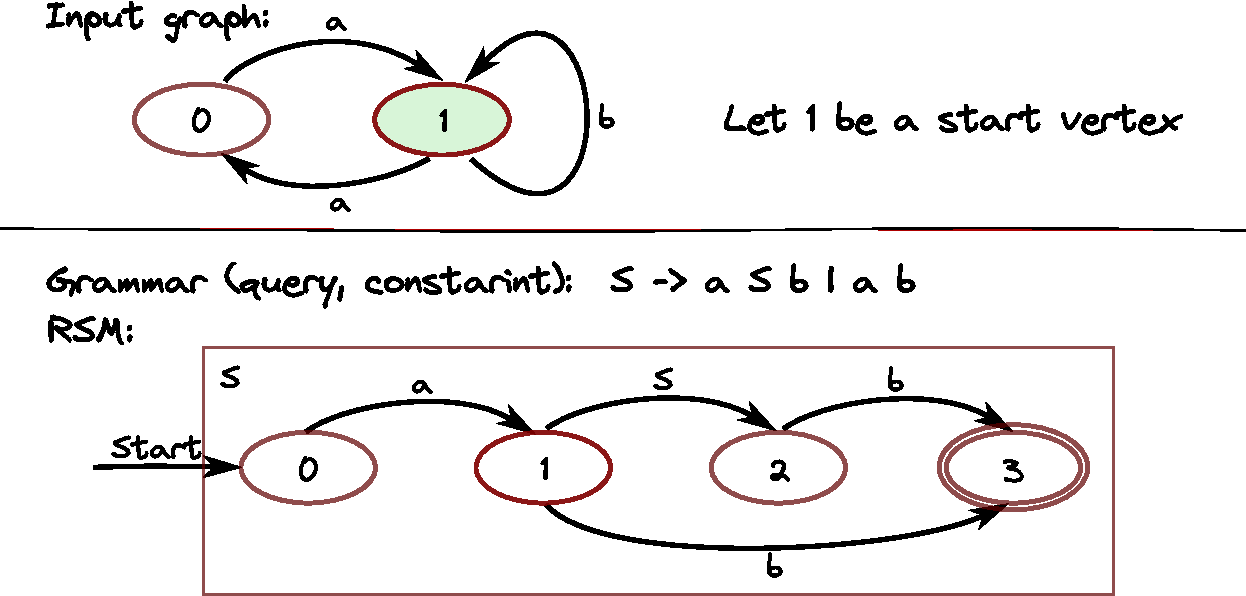
\includegraphics[width=0.99\textwidth]{pictures/RSM.pdf}
  \end{center}
\end{frame}

\begin{frame}[fragile] \frametitle{Generalized LL for CFPQ: The Idea}
  \begin{center}
      \includegraphics[width=0.99\textwidth]{pictures/gll.pdf}
  \end{center}
\end{frame}

\begin{frame}[fragile] \frametitle{SPPF is a Representation of All Paths of Interest}
  \begin{center}
      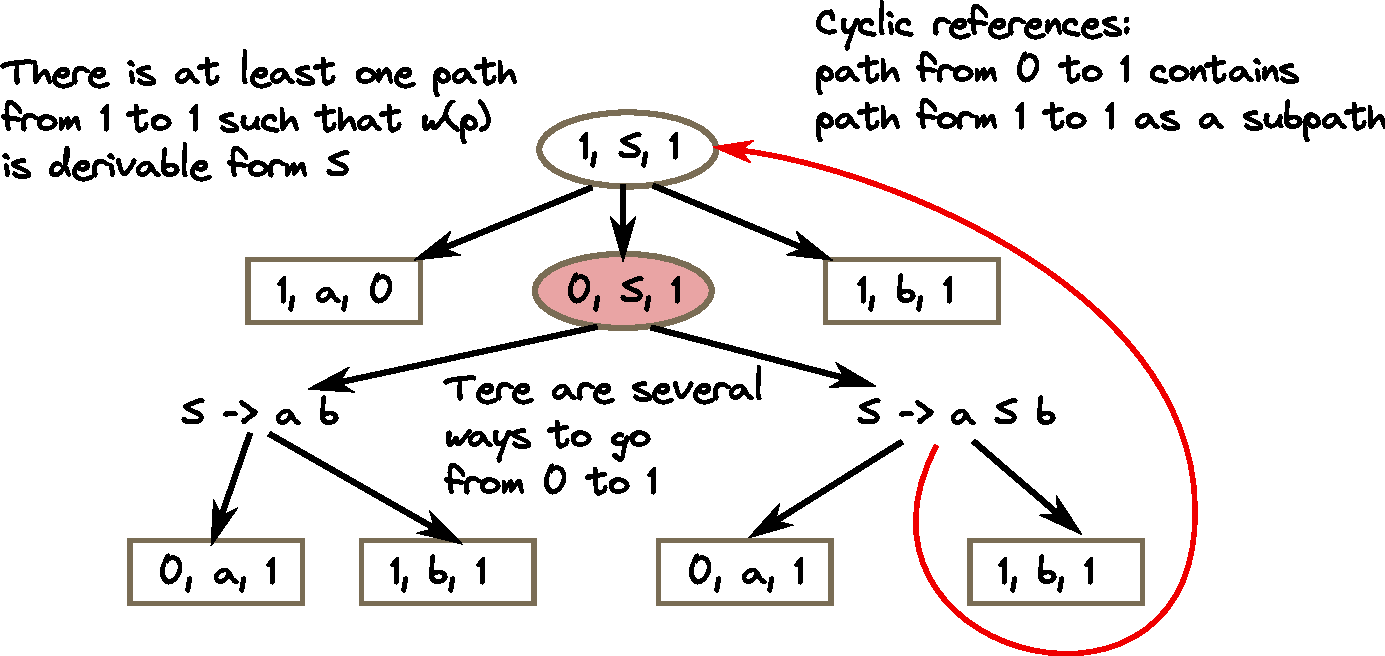
\includegraphics[width=0.89\textwidth]{pictures/sppf.pdf}
  \end{center}
\end{frame}


\begin{frame}[fragile] \frametitle{Trees And Paths}
  \begin{center}
      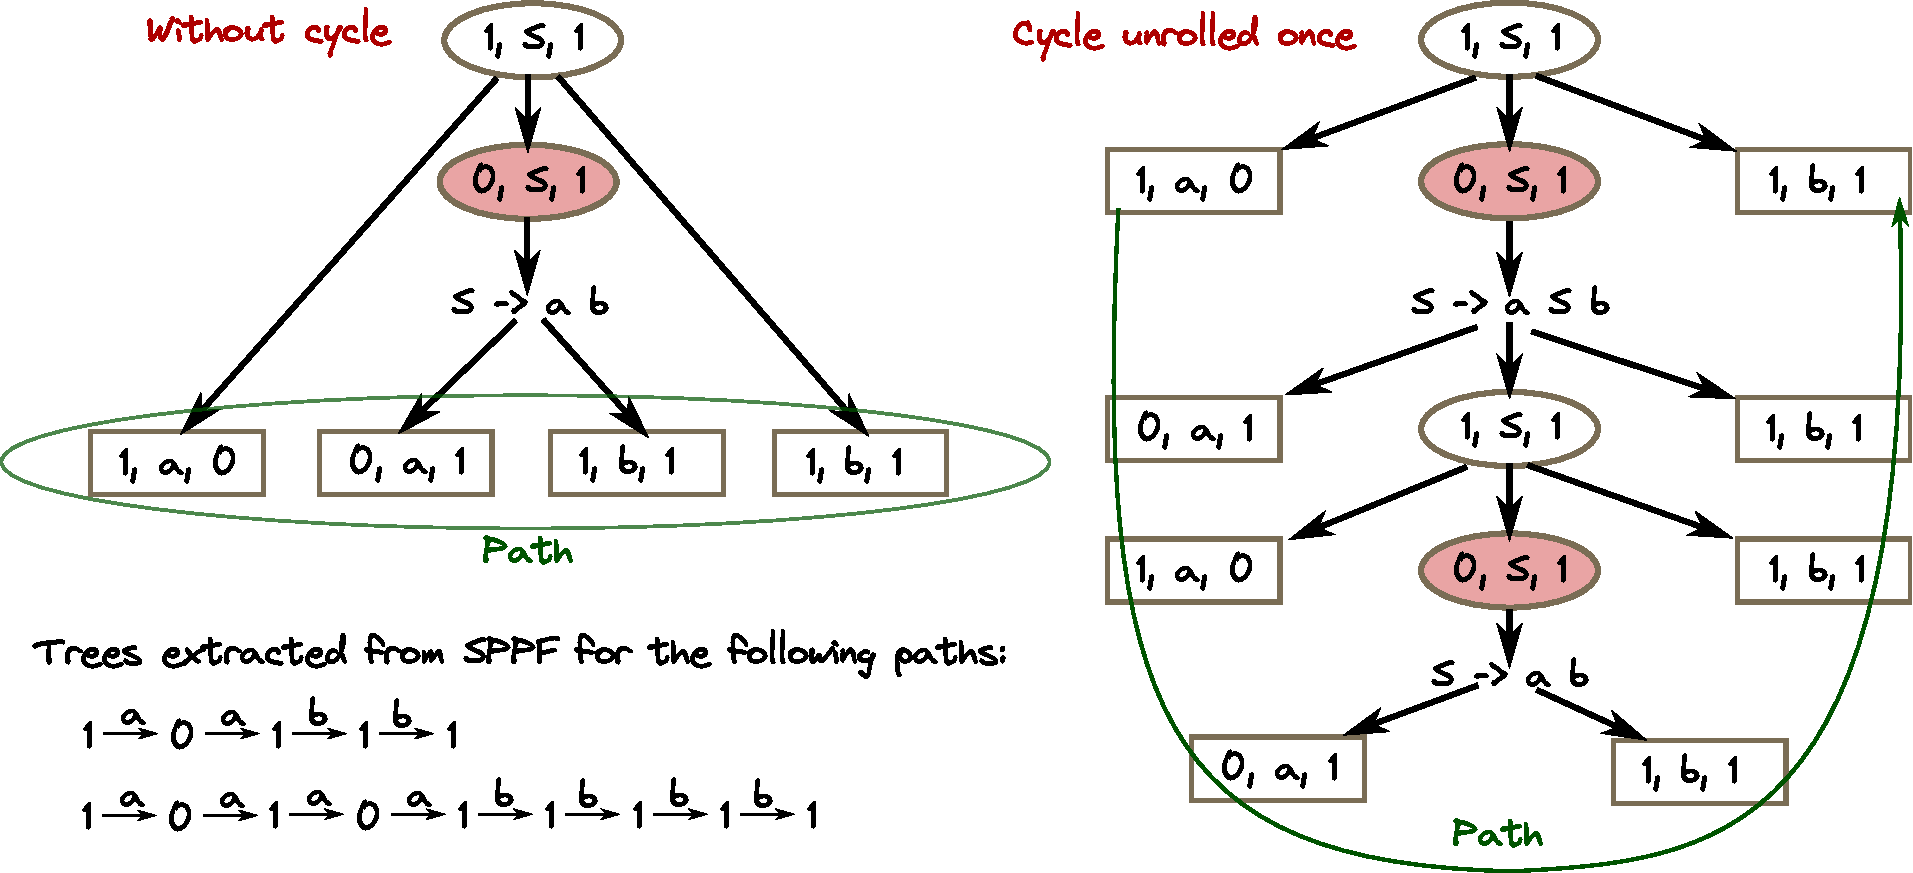
\includegraphics[width=0.99\textwidth]{pictures/Trees.pdf}
  \end{center}
\end{frame}


\begin{frame}[fragile] \frametitle{Context-Free Languages Are Closed Under Intersection With Regular Ones}
  \begin{center}
      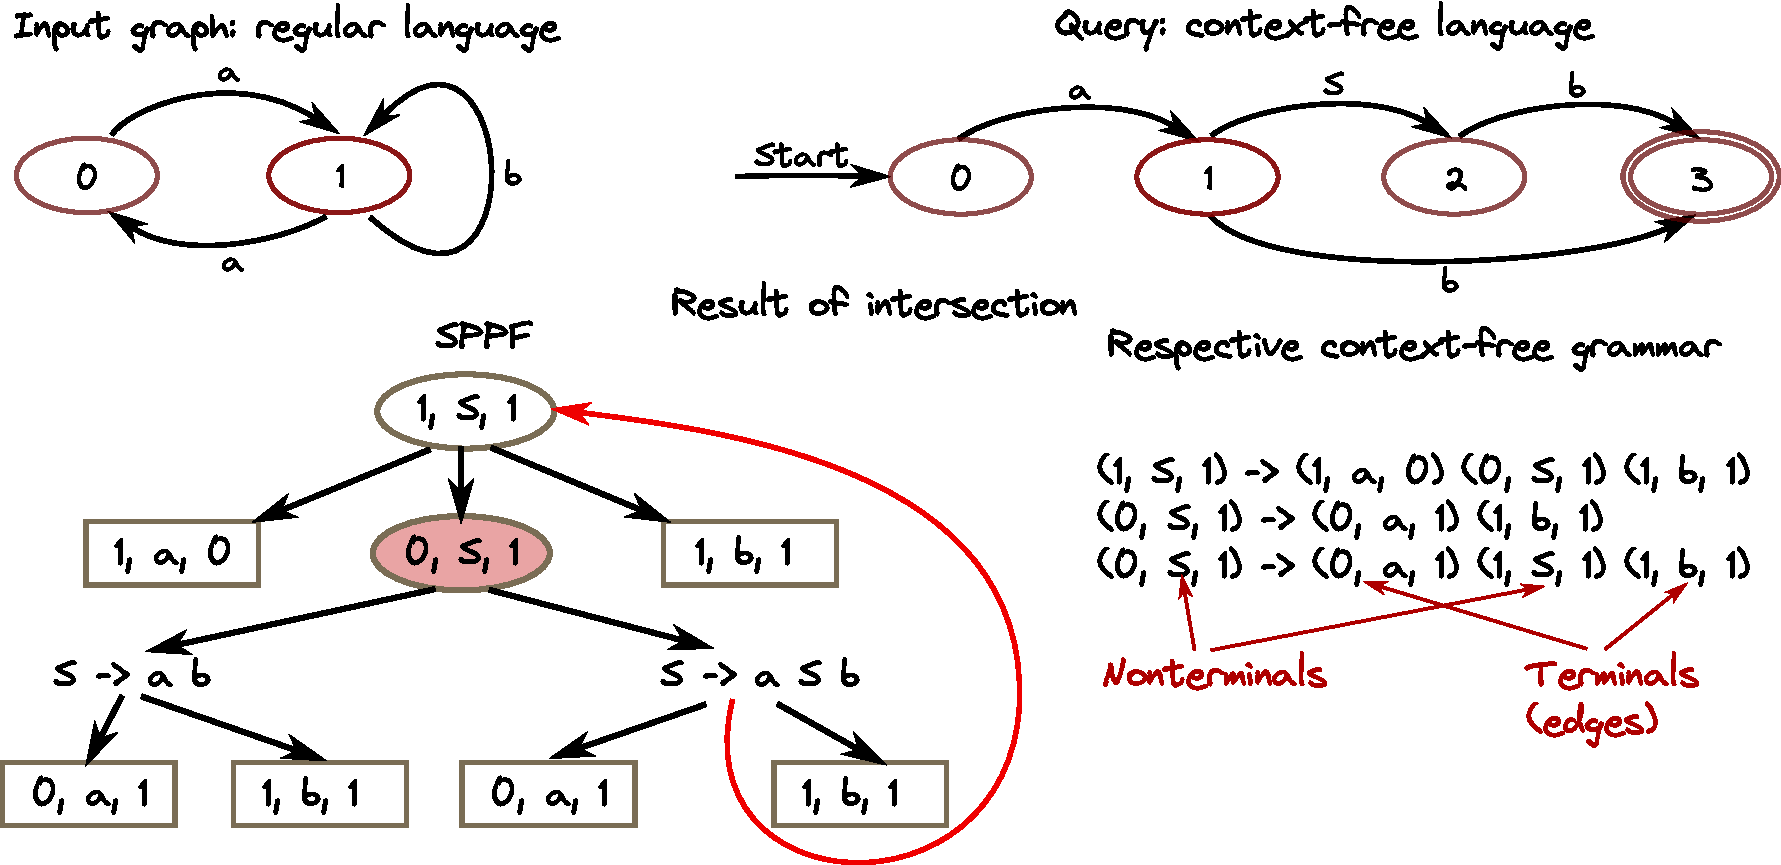
\includegraphics[width=0.99\textwidth]{pictures/Intersection.pdf}
  \end{center}
\end{frame}


%\begin{frame}[fragile] \frametitle{Recursive State Machine}  
%\begin{tikzpicture}[thick,scale=1.0, node distance=\nodeDistanceRsm,
%                    shorten >=1pt,on grid,auto] 
%
%  \node[state, initial left] (q_0)   {$q_0$};
%  \node[state] (q_1) [above right=of q_0] {$q_1$};
%  \node[state] (q_2) [right=of q_1] {$q_2$};
%  \node[state, accepting] (q_3) [below right=of q_2] {$q_3$};
%  \node[state] (q_4) [below right=of q_0] {$q_4$};
%  \node[state] (q_5) [right=of q_4] {$q_5$};
%
%  \node[draw=black, fit=(q_0) (q_1) (q_5) (q_3), inner xsep=0.1cm, inner ysep=0.1cm] (E) {};
%  \node[below right] at (E.north west) {S};
%
%  \path[->]
%    (q_0) edge[sloped, right, above, bend left] node {$\overline{subClassOf}$} (q_1)
%    (q_1) edge node {$q_0$} (q_2)
%    (q_2) edge[sloped, right, above, bend left] node {$subClassOf$} (q_3)
%    (q_1) edge[sloped, above] node {$subClassOf$} (q_3)
%    (q_0) edge[bend right, sloped, below] node {$\overline{type}$} (q_4)
%    (q_4) edge[below] node {$q_0$} (q_5)
%    (q_5) edge[left, sloped, bend right, below] node {$type$} (q_3)
%    (q_4) edge[sloped, above] node {$type$} (q_3);
%\end{tikzpicture}
%\end{frame}




\begin{frame}[fragile] \frametitle{Implementation Details}
  \begin{itemize}
  \item Generic CFPQ solver (graph is abstraction)
  \item Neo4j as graph storage (no Cypher extension to support CFPQ)  
  \end{itemize}
\end{frame}


\begin{frame}[fragile] \frametitle{Evaluation Setup}

\begin{minipage}[t]{0.51\textwidth}
\vspace{-1.4cm}
\begin{itemize}
  \item Ubuntu 20.04, Intel Core i7-6700 CPU, 3.4GHz, DDR4 64Gb RAM
  \item Neo4j 5.12.0
  \begin{itemize}
    \item Unlimited memory usage per transaction
  \end{itemize}
  \item JVM was configured to use 55Gb  
\end{itemize}

\end{minipage}
~
\begin{minipage}[t]{0.44\textwidth}
{
\resizebox{1.1\textwidth}{!}{
\rowcolors{2}{black!2}{black!10}
\begin{tabular}{| l | c | c | c | c | c |}
         \hline
         Graph name & $|V|$ & $|E|$ & \#subClassOf & \#type \\
         \hline
         \hline
         Core               & 1 323     & 2 752      & 178        & 0         \\
         Pathways           & 6 238     & 12 363     & 3 117      & 3 118     \\
         Go\_hierarchy       & 45 007    & 490 109    & 490 109    & 0        \\
         Enzyme             & 48 815    & 86 543     & 8 163      & 14 989    \\
         Eclass             & 239 111   & 360 248    & 90 962     & 72 517    \\
         Geospecies         & 450 609   & 2 201 532  & 0          & 89 065    \\
         Go                 & 582 929   & 1 437 437  & 94 514     & 226 481   \\
         Taxonomy           & 5 728 398 & 14 922 125 & 2 112 637  & 2 508 635 \\
         \hline
    \end{tabular}
}
}
\end{minipage}

Queries:
\begin{align*}
&Q_1: & S \to & \overline{\textit{subClassOf}} \ \ S \ \textit{subClasOf} \mid \overline{\textit{type}} \ \ S \ \textit{type} \\ 
&     &       & \mid \overline{\textit{subClassOf}} \ \ \textit{subClassOf} \mid \overline{\textit{type}} \ \textit{type} \\
&Q_2: & S  \to & \overline{\textit{subClassOf}} \ \ S \ \textit{subClasOf} \mid \textit{subClassOf} \\
&\textit{reg}_1:& S  \to  & (\textit{subClassOf} \mid \textit{type})^* \\
&\textit{reg}_2:& S  \to  & \textit{subClassOf }^* \cdot \textit{type}^*
\end{align*}

\end{frame}


\begin{frame}[fragile] \frametitle{CFPQ reachability speedup (RSM over CFG) on RDF graphs}  
  \begin{center}   
    $Q_1$ \hspace{7cm} $Q_2$     \\
    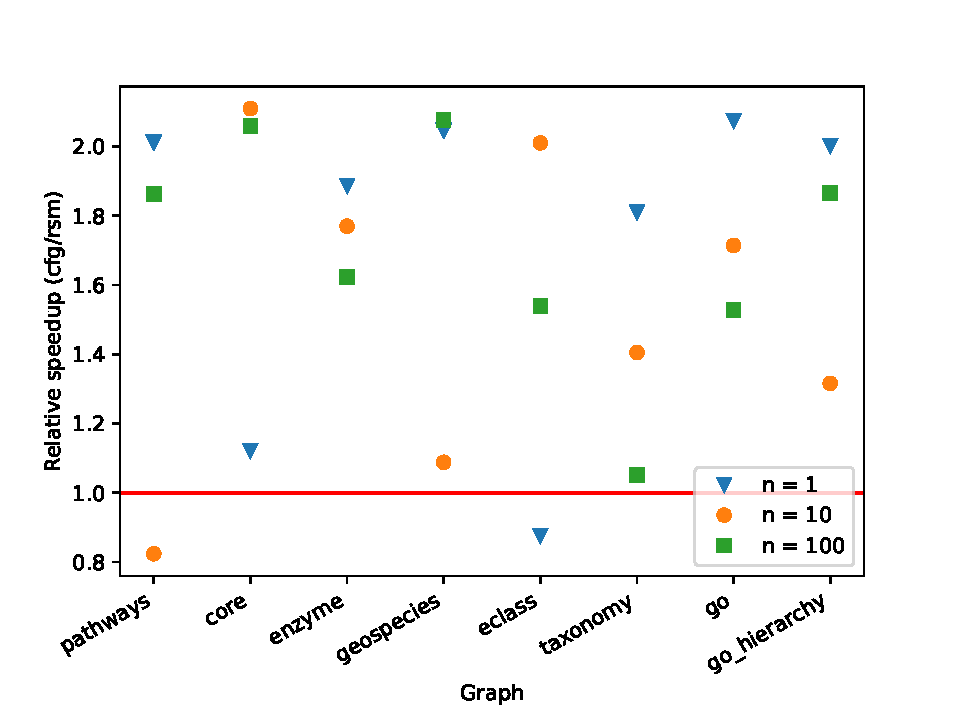
\includegraphics[width=0.49\textwidth]{pictures/g1_kotgll_result.pdf}
    %\caption{ $G_1$ query}            
    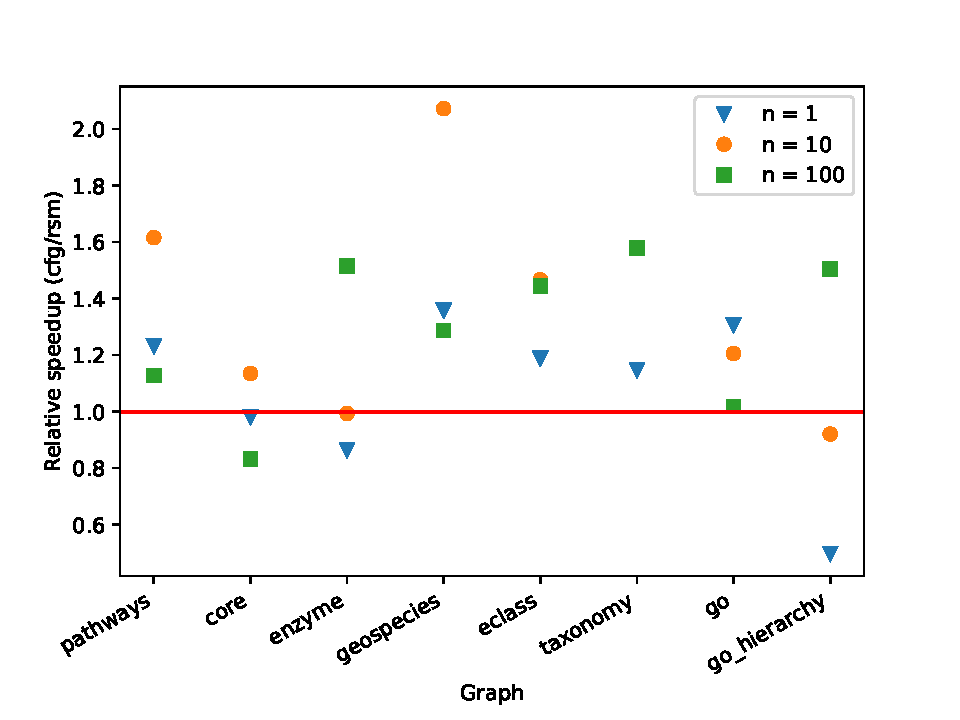
\includegraphics[width=0.49\textwidth]{pictures/g2_kotgll_result.pdf}
    %\caption{$G_2$ query}        
    %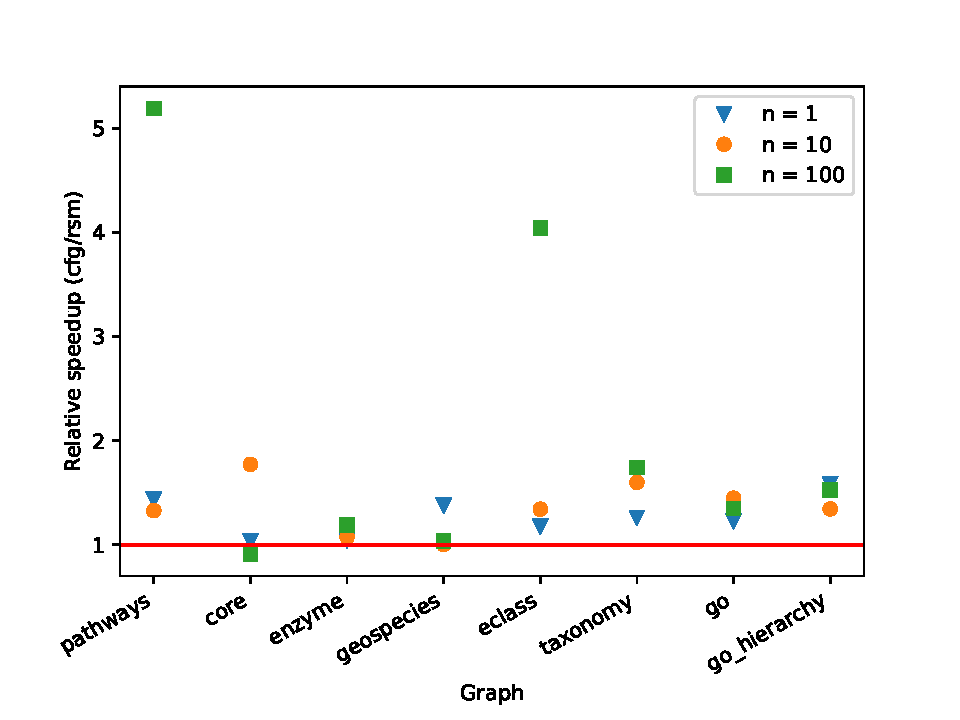
\includegraphics[width=0.49\textwidth]{pictures/geo_kotgll_result.pdf}
    %\caption{$Geo$ query}
  \end{center}
\end{frame}


\begin{frame}[fragile] \frametitle{CFPQ results (Neo4j vs RedisGraph)}
  \begin{center}
    $Q_1$ \hspace{7cm} $Q_2$     \\
    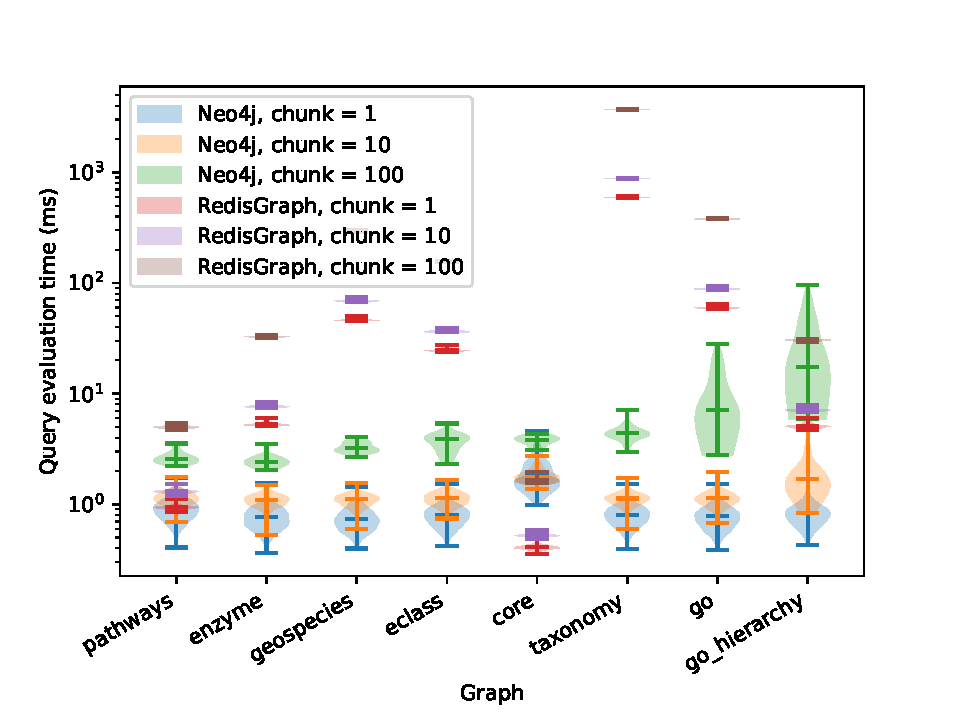
\includegraphics[width=0.49\textwidth]{pictures/g1_result.pdf}
    %\caption{ $G_1$ query}            
    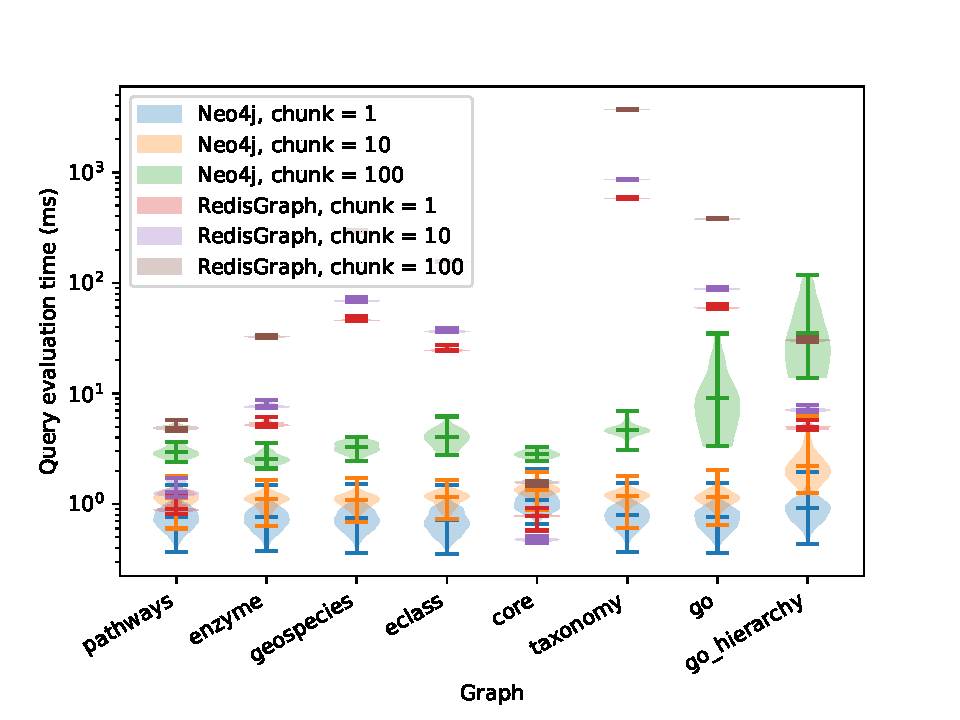
\includegraphics[width=0.49\textwidth]{pictures/g2_result.pdf}
    %\caption{$G_2$ query}        
    %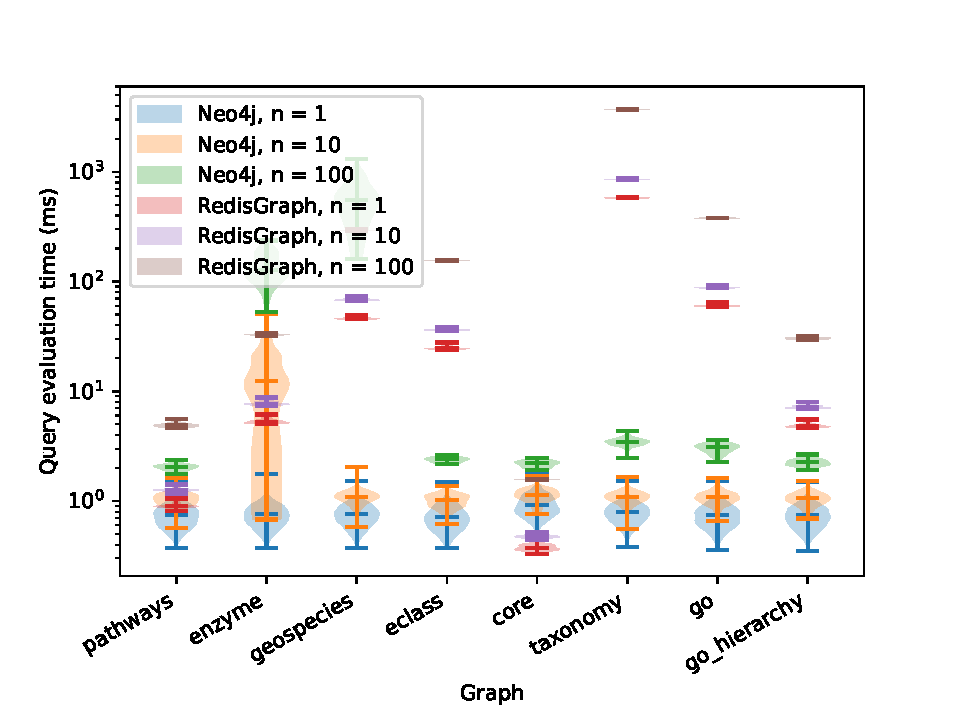
\includegraphics[width=0.49\textwidth]{pictures/geo_result.pdf}
    %\caption{$Geo$ query}
  \end{center}
\end{frame}

\begin{frame}[fragile] \frametitle{RPQ results for Neo4j\footnote{Native solution failed with OOM on last two graphs}}
  \begin{center}
    $\textit{reg}_1$ \hspace{7cm} $\textit{reg}_2$     \\
    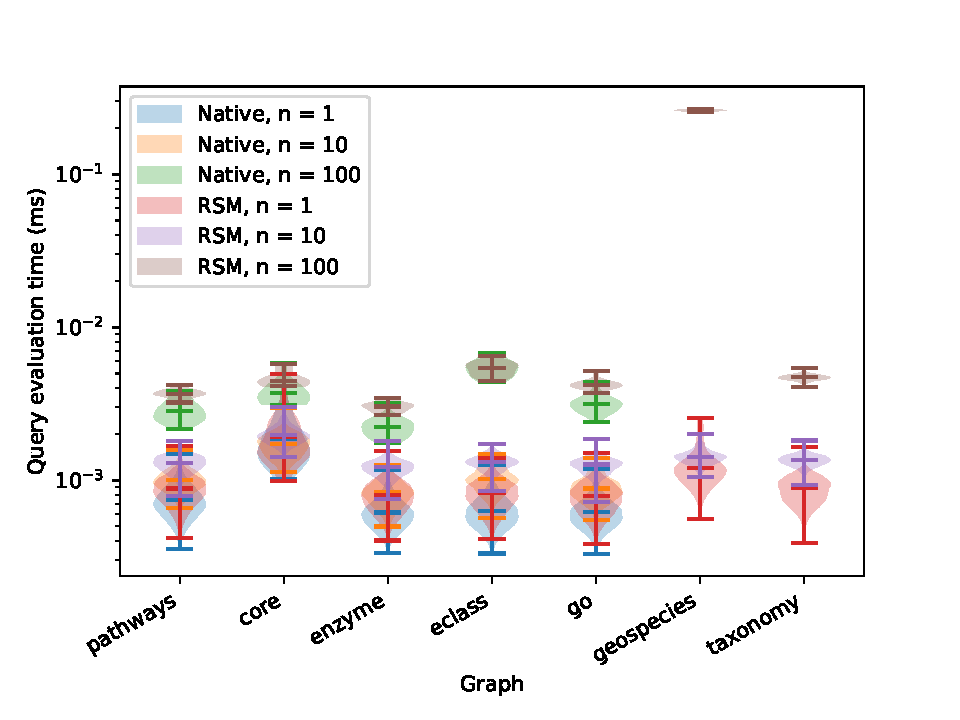
\includegraphics[width=0.49\textwidth]{pictures/reg1_rpq_result.pdf}
    %\caption{ $G_1$ query}            
    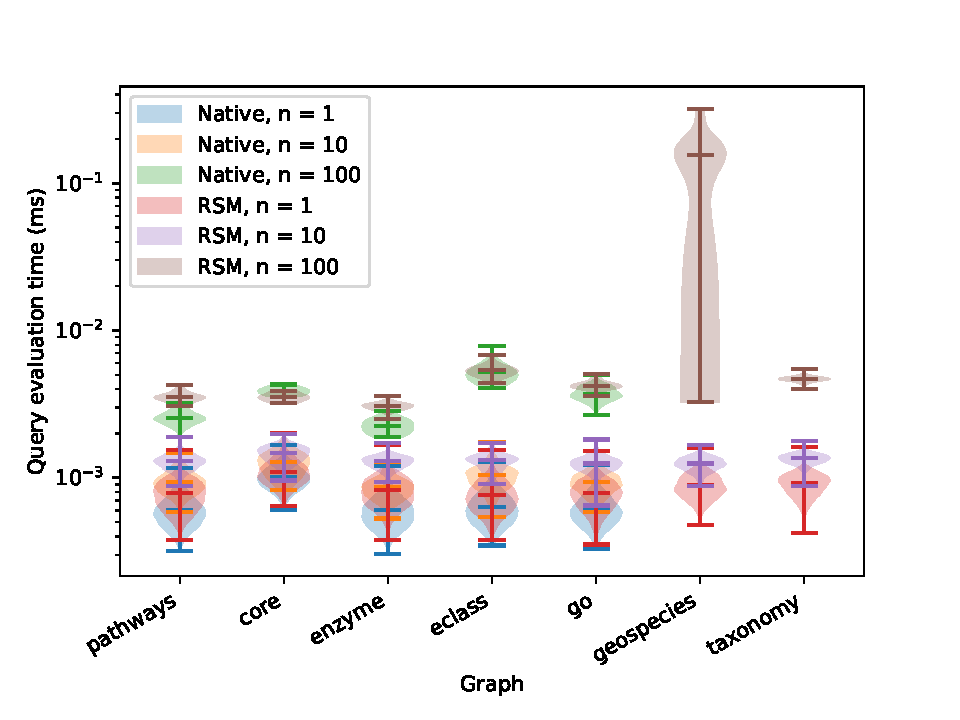
\includegraphics[width=0.49\textwidth]{pictures/reg2_rpq_result.pdf}
    %\caption{$G_2$ query}        
    %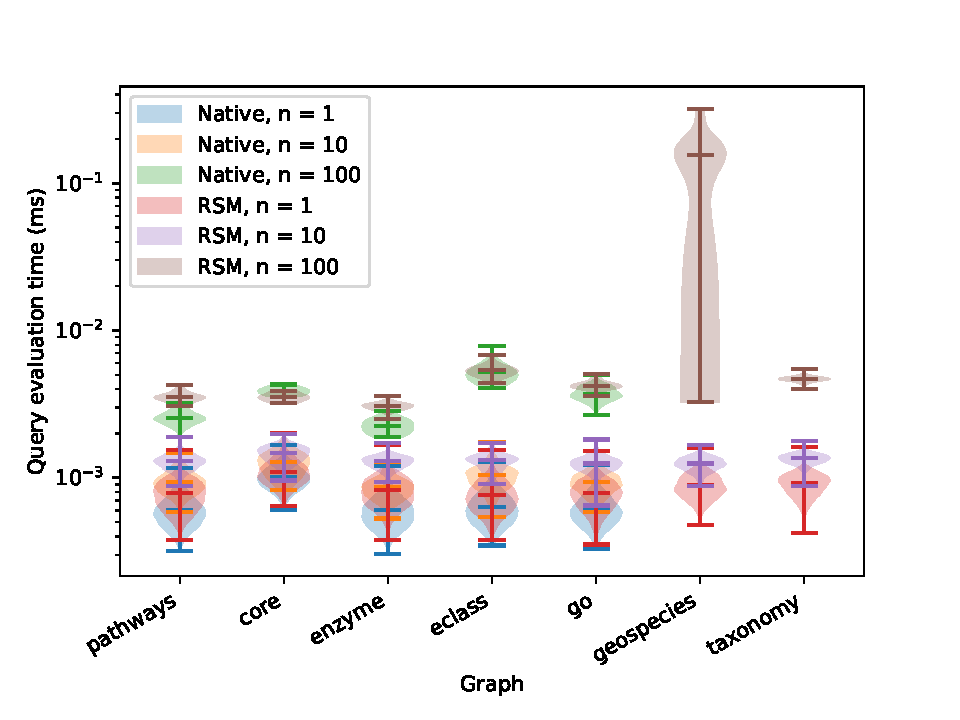
\includegraphics[width=0.49\textwidth]{pictures/reg2_rpq_result.pdf}
    %\caption{$Geo$ query}
  \end{center}
\end{frame}

\begin{frame}[fragile] \frametitle{Conclusion And Future Research}
  \begin{itemize}
      \item[\faCheck] GLL-based CFPQ algorithm 
      \begin{itemize}
         \item RSM is promising representation of CFLs in context of CFPQ
         \item In some cases faster than linear-algebra-based approach
         \item Comparable with native RPQ (for Neo4j)
      \end{itemize}
      \item[\faGears] Implementation of paths extraction strategies
      \item[\faHourglassStart] Parallel version of GLL
      \begin{itemize}
         \item[\faLightbulbO] All descriptors can be handled independently
         \item[\faFrownO] Complex global shared structures (GSS, SPPF, etc) --- synchronization needed
      \end{itemize}      
      \item[\faHourglassStart] Incremental version of GLL
  \end{itemize}
\end{frame}

%\begin{frame}
%\frametitle{Contact Information}
%\begin{minipage}[t]{0.8\textwidth}
%\begin{itemize}
%  \item Try it out (Docker image with extended RedisGraph): \url{https://hub.docker.com/r/simpletondl/redisgraph}
%  \item RedisGraph extended with CFPQ: \url{https://github.com/YaccConstructor/RedisGraph}
%  \item Cypher parser extended with path patterns: \url{https://github.com/YaccConstructor/libcypher-parser}
%
%  \vspace{0.5cm}
%  \pause
%  \item Semyon Grigorev: \href{mailto:s.v.grigoriev@spbu.ru}{s.v.grigoriev@spbu.ru}
%  \item Arseniy Terekhov: \href{mailto:simpletondl@yandex.ru}{simpletondl@yandex.ru}
%  \item Vlada Pogozhelskaya: \href{mailto:pogozhelskaya@gmail.com}{pogozhelskaya@gmail.com}
%  \item Vadim Abzalov: \href{mailto:vadim.i.abzalov@gmail.com}{vadim.i.abzalov@gmail.com}
%  \item Timur Zinnatulin: \href{mailto:teemychteemych@gmail.com}{teemychteemych@gmail.com}
%\end{itemize}
%\end{minipage}~
%\begin{minipage}[t]{0.19\textwidth}
%\pause
%\vspace{2.5cm}
%\center{\huge{Thanks!}}
%\end{minipage}
%\end{frame}

\end{document}
